\section{Speed Measurements} \label{sec:measurements-speed}
In this chapter the generated data with CPlan \ref{CPlan} is compared and analysed.

\begin{figure}
    \centering
    \begin{mdframed}[style=mdthight]
        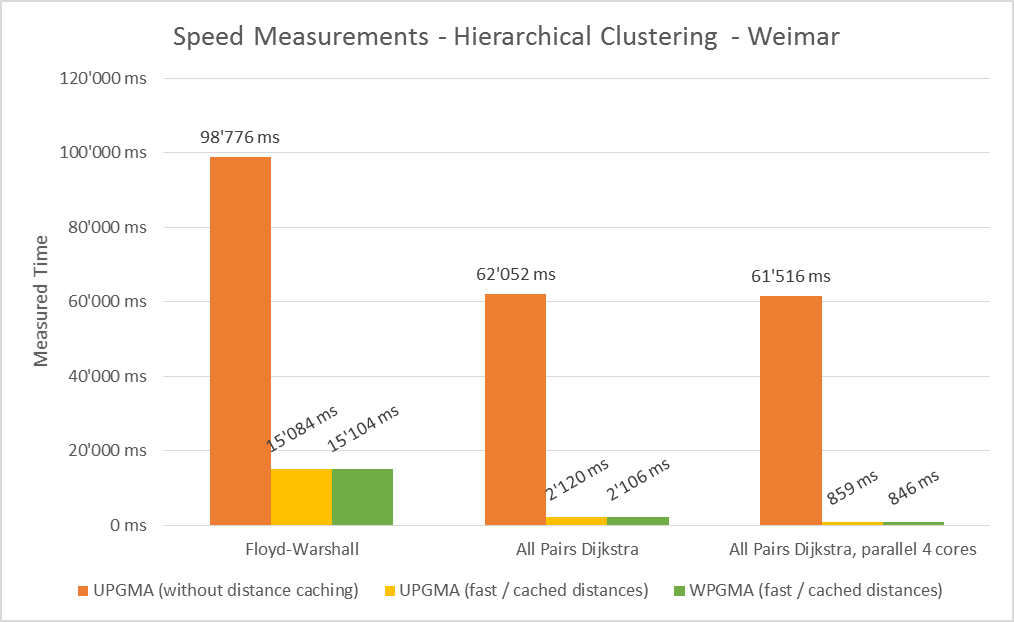
\includegraphics[width=\textwidth]{hierarchical_clustering_speed.png}
    \end{mdframed}
    \caption{\label{fig:hierarchical_clustering_speed}}
\end{figure}

\begin{figure}
    \centering
    \begin{mdframed}[style=mdthight]
        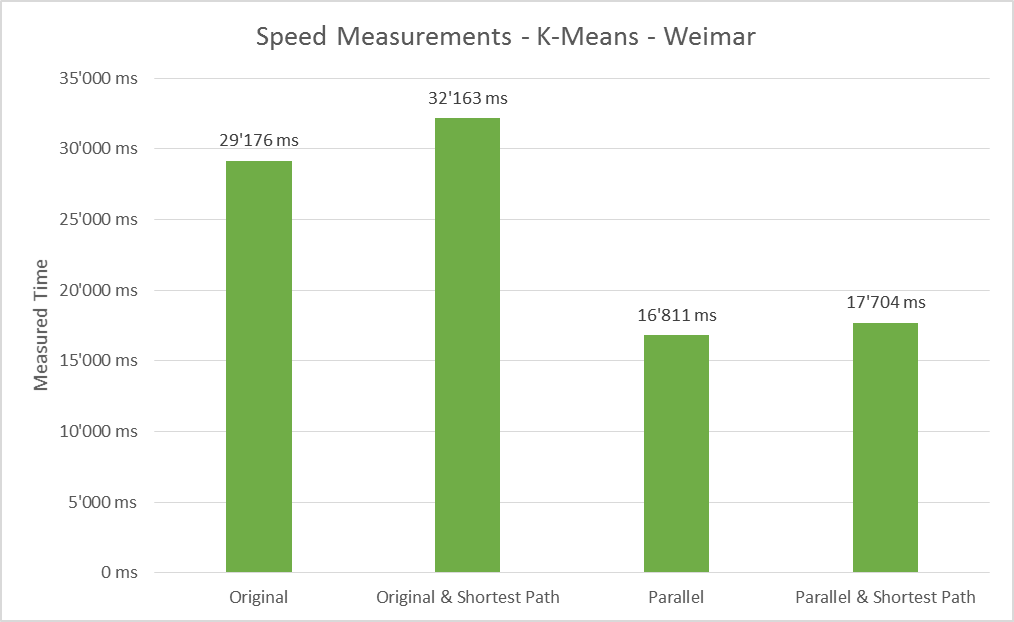
\includegraphics[width=\textwidth]{kmeans_speed.png}
    \end{mdframed}
    \caption{\label{fig:kmeans_speed}}
\end{figure}

TODO: Description of speed measurements here. 

TODO: Table of speed measurements here.

\pagebreak
\section{Cluster Analysis}
\label{sec:measurements-cluster-analysis}
In this chapter the provided measurement methods \ref{sec:clusterRating} are used to compare the measured results between the different districts/areas. The following images were generated with the cluster algorithm FastUPGMA \ref{sec:UPGMAandWPGMA} on Weimar with \textit{Modified Output} and \textit{Number of Clusters} count 16.

A example for every district from the chapter \ref{sec:concept_cluster_analysis} was found. Three different colours can be observed. Red labelled edges are within the cluster. Grey edges are transitions between different clusters and black edges are outside of the cluster.

As expected in section \ref{sec:historyDistinct} the historic subgraph (figure \ref{fig:result_historic_district}) had a high block count on a small area. The street count, the vertex connections mean and the density are high. All results for this cluster can be viewed in table \ref{tab:measured_cluster_ratings} cluster number c1.

\begin{figure}[ht]
    \centering
    \begin{mdframed}[style=mdthight, userdefinedwidth=0.4\textwidth, align=center]
        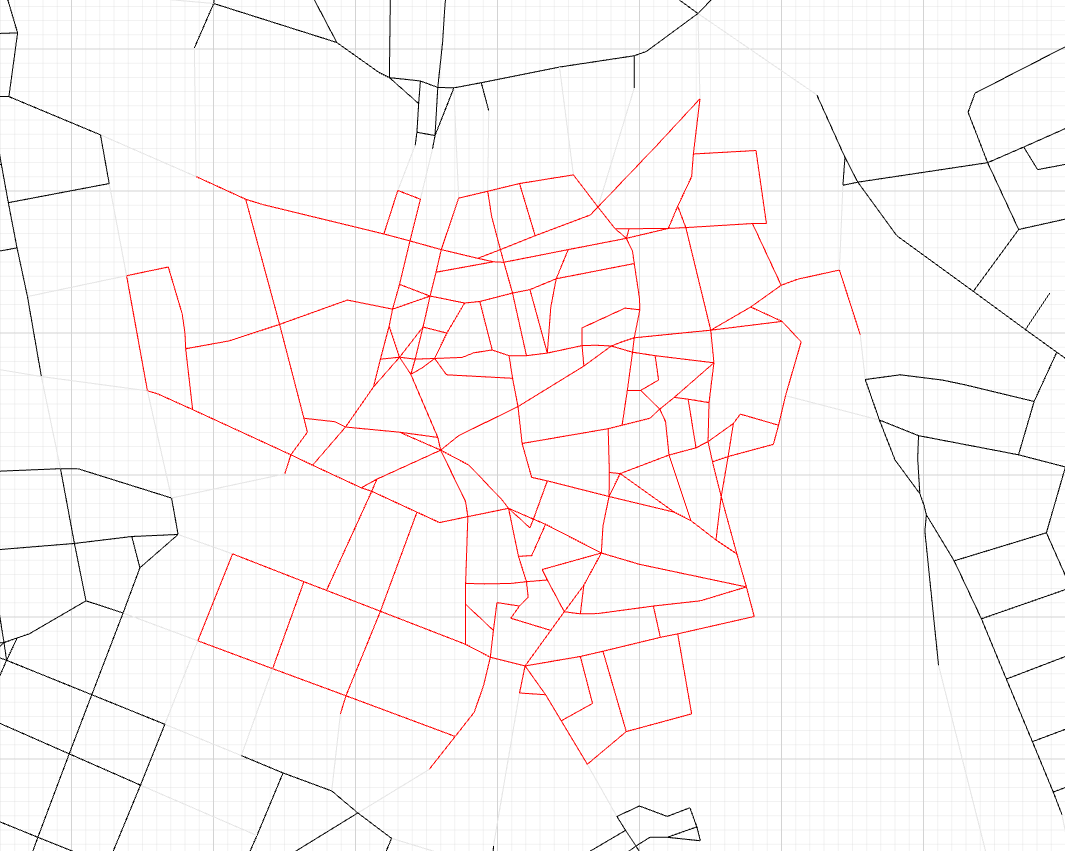
\includegraphics[width=\linewidth]{district_result_historic.png}
    \end{mdframed}
    \caption{Historic District Subgraph}
    \label{fig:result_historic_district}
\end{figure}
\FloatBarrier

Like anticipated in section \ref{sec:businessDistinct} the business district (figure \ref{fig:result_business_district}) had the highest relative block area (A/Ac) and a very high integration value. The mean connection count and the density are much higher compared with the historic district. This insights can be observed in table \ref{tab:measured_cluster_ratings} cluster number C2.

\begin{figure}[ht]
    \centering
    \begin{mdframed}[style=mdthight, userdefinedwidth=0.4\textwidth, align=center]
        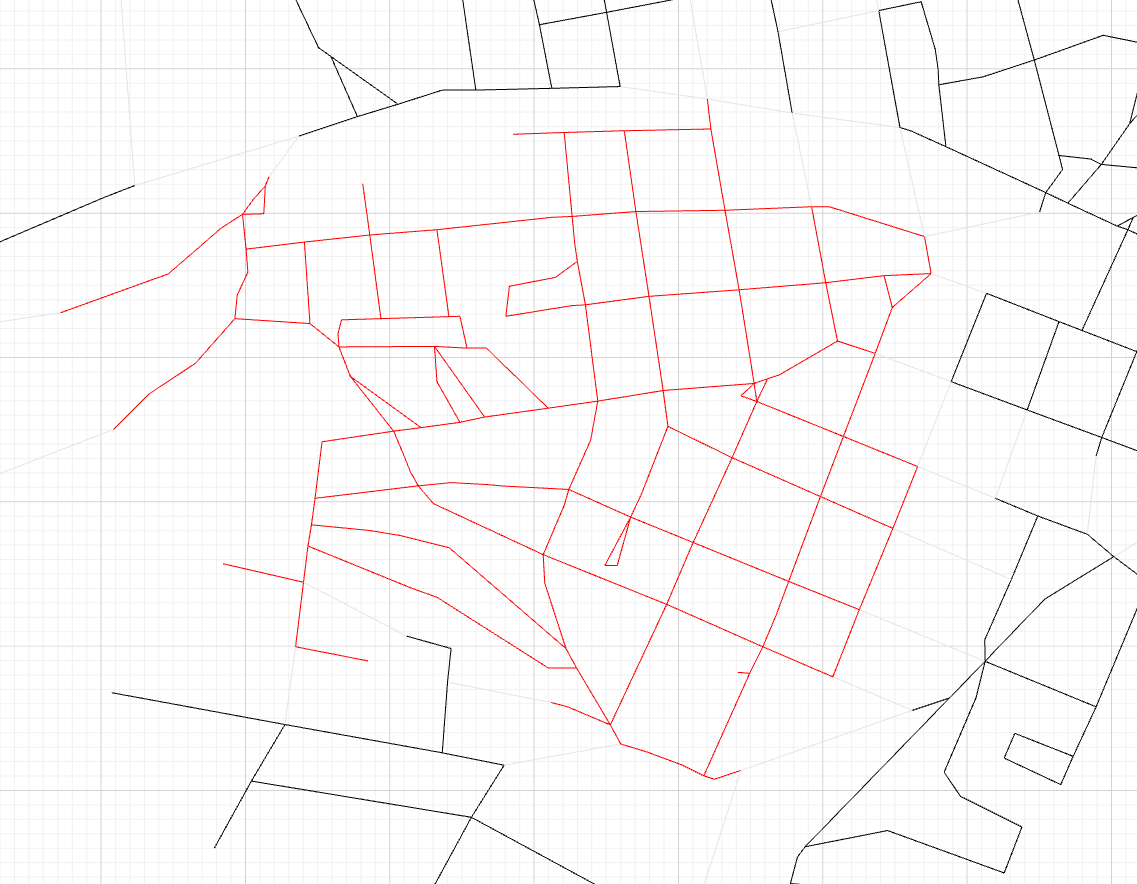
\includegraphics[width=\linewidth]{district_result_business.png}
    \end{mdframed}
    \caption{Business District Subgraph}
    \label{fig:result_business_district}
\end{figure}
\FloatBarrier

A detected outskirts subgraph can be viewed in figure \ref{fig:result_outskirts_district}. The measured results can be found in table \ref{tab:measured_cluster_ratings} cluster number C3. They show as expected a high street length variance and median. The density is very high because of a low street count on a big area.

\begin{figure}[ht]
    \centering
    \begin{mdframed}[style=mdthight, userdefinedwidth=0.6\textwidth, align=center]
        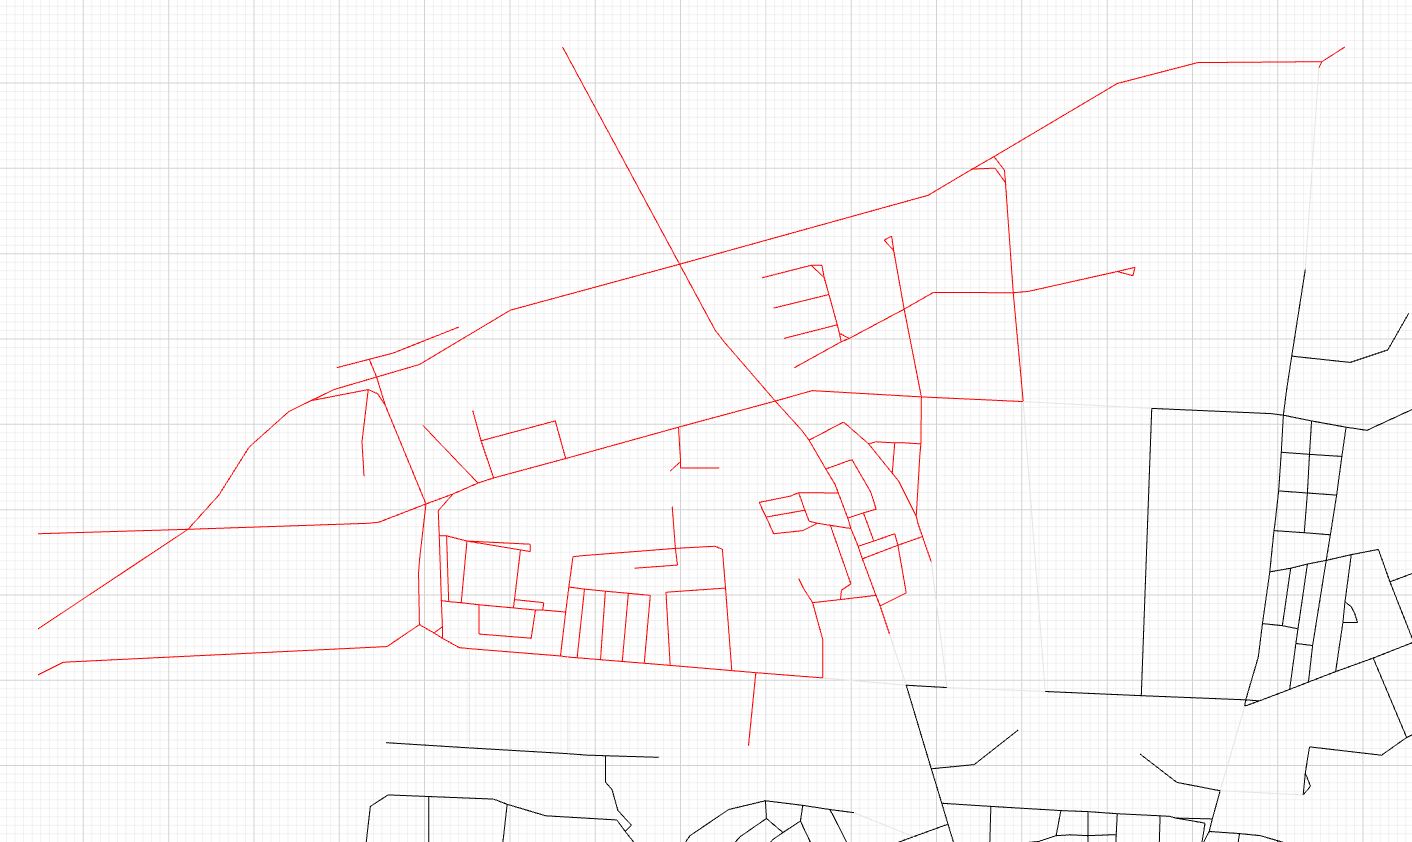
\includegraphics[width=\linewidth]{district_result_outskirts.png}
    \end{mdframed}
    \caption{Outskirts Subgraph}
    \label{fig:result_outskirts_district}
\end{figure}
\FloatBarrier

\FloatBarrier
\subsection{Measured Data}
\label{sec:ClusterAnalysisMeasurements}
The following table \ref{tab:cluterAnalysisDescription} contains the parameters with additional descriptions. Of every parameter the minimal (min), maximal (max), mean (average) and the median value can be calculated. Because the min, max values don't have any relevance they were skipped in this table. All measurements can be observed in the appendix in \ref{sec:measurements_full_table}.

\begin{table}[!ht]
\centering
\begin{tabular}{ | l | l |} \hline 
    \textbf{Parameter} & \textbf{Description} \\
    \hline
    Total Area &  Area of the convex hull \\ \hline
    Total Length & Sum of the street length \\ \hline
    Density & 'Total Area' divided by 'Total Length'  \\ \hline
    
    Street Length Min/Max/Mean & Shortest/Longest/Average street length  \\ \hline
    Street Length Median & Middle value of the length dataset \\ \hline
    Street Length Variance & Sigma of the normal distribution curve of the variance \\ \hline
    
    Vertex Connections & Mean connected edges per vertex  \\ \hline
    
    Street Angle Min/Max/Mean & Smallest/Biggest/Average angle between two edges \\ \hline
    Street Angle Variance & Sigma of the normal distribution curve of the angles \\ \hline
    
    Block Count & Total number of blocks \\ \hline
    Block Area Min/Max/Mean & Shortest/Biggest/Average block area \\ \hline
    Block Area A/Ac Min/Max/Mean & Block area divided to a minimal circle around a block \\ \hline
    
    Integration Min/Max/Mean & Normalised In-Centrality \\ \hline
    Choice Min/Max/Mean & Normalised In-Betweenness-Centrality \\ \hline
\end{tabular}
\caption{Parameter with descriptions for table \ref{tab:measured_cluster_ratings}}
\label{tab:cluterAnalysisDescription}
\bigskip
\bigskip
\centering
\begin{tabular}{ |l|l|l|l|l| }
    \hline
    \textbf{Parmate}r &
    & \textbf{C1} \ref{sec:historyDistinct}
    & \textbf{C2} \ref{sec:businessDistinct}
    & \textbf{C3} \ref{sec:outskits}  \\ 
    \hline
    \multirow{4}{*}{Total} 
    & Area & 1838.05 & 1956.59 & 7802.74 \\
    & Length & 806.92 & 643.50 & 1069.81 \\
    & Density & 2.28 & 3.04 & 7.29 \\
    \hline
    \multirow{3}{*}{Street Length}
    & Mean & 2.72 & 3.85 & 4.82 \\
    & Median & 2.30 & 3.65 & 3.28 \\
    & Variance & 1.70 & 2.19 & 5.00 \\
    \hline
    \multirow{1}{*}{Vertex} 
    & Connections & 3.04 & 2.84 & 2.45 \\
    \hline
    \multirow{2}{*}{Street Angle} 
    & Mean & 119.03 & 123.75 & 137.18 \\
    & Variance & 124.68 & 131.65 & 129.47 \\
    \hline
    \multirow{3}{*}{Block} 
    & Count & 55 & 35 & 26 \\
    & Area Mean & 6.54 & 13.65 & 76.30 \\
    & A/Ac Mean & 0.18 & 0.23 & 0.18 \\
    \hline
    \multirow{1}{*}{Integration} 
    & Mean & 0.49 & 0.59 & 0.78 \\
    \hline
    \multirow{1}{*}{Choice}
    & Mean & 0.10 & 0.05 & 0.04 \\
    \hline
\end{tabular}
\caption{Measured results from Historic District (C1) \ref{sec:historyDistinct}, Business District (C2) \ref{sec:businessDistinct} and Outskirts Area (C3) \ref{sec:outskits}}
\label{tab:measured_cluster_ratings}

\end{table}
